\chapter{Parametri del modello ``dializzatore''}\label{app:B}



\section{Dialisance/Clearance}
Il filtro utilizzato nel centro dialisi per le sedute di \textit{on-line} HDF è il filtro \textit{Fresenius} HF80s, le cui caratteristiche di clearance sono tabulate in \tablename~\ref{tab:CL} in base al peso molecolare $PM$ e alla portata $Q_B$ di sangue intero in ingresso al dializzatore, in regime di filtrazione nulla.
\begin{table}[htb]
	\centering
	\caption{Clearance di alcuni soluti. Filtro \textit{Fresenius HF80s}, $Q_f=0.$}\label{tab:CL}
	\begin{tabular}{lrcc}
	\toprule 
		\textbf{Soluto}   & \textbf{PM} & \multicolumn{2}{c}{\textbf{Clearance} $\mathbf{(mL/min)}$}  \\
		\cmidrule(lr){3-4}
		                  &             & $(Q_B=200$ $mL/min)$ & $(Q_B=300$ $mL/min)$ \\
  \midrule
  	Urea              & $60$        & $192$               & $248$               \\
  	Creatinina        & $113$       & $180$               & $225$               \\
  	Vitamina $B_{12}$ & $1355$      & $135$               & $155$               \\
  	Inulina           & $5200$      & $110$               & $120$               \\
  \bottomrule
\end{tabular}
\end{table}
Il valore di clearance/dialisance per i soluti di interesse (sodio, potassio, \ldots) è calcolato in base a una doppia interpolazione dei valori di \tablename~\ref{tab:CL}: la prima interpolazione di tipo logaritmica, in base al peso molecolare; la seconda lineare in base alla portata volumetrica in ingresso al dializzatore. A titolo esemplificativo, in \figurename\ref{fig:doppia_interp} mostriamo con una linea nera tratteggiata il risultato della doppia interpolazione per una vasta gamma di pesi molecolari quando in ingresso al dializzatore si ha una portata di $250$ $mL/min$.
\begin{figure}[htb]
	\centering
		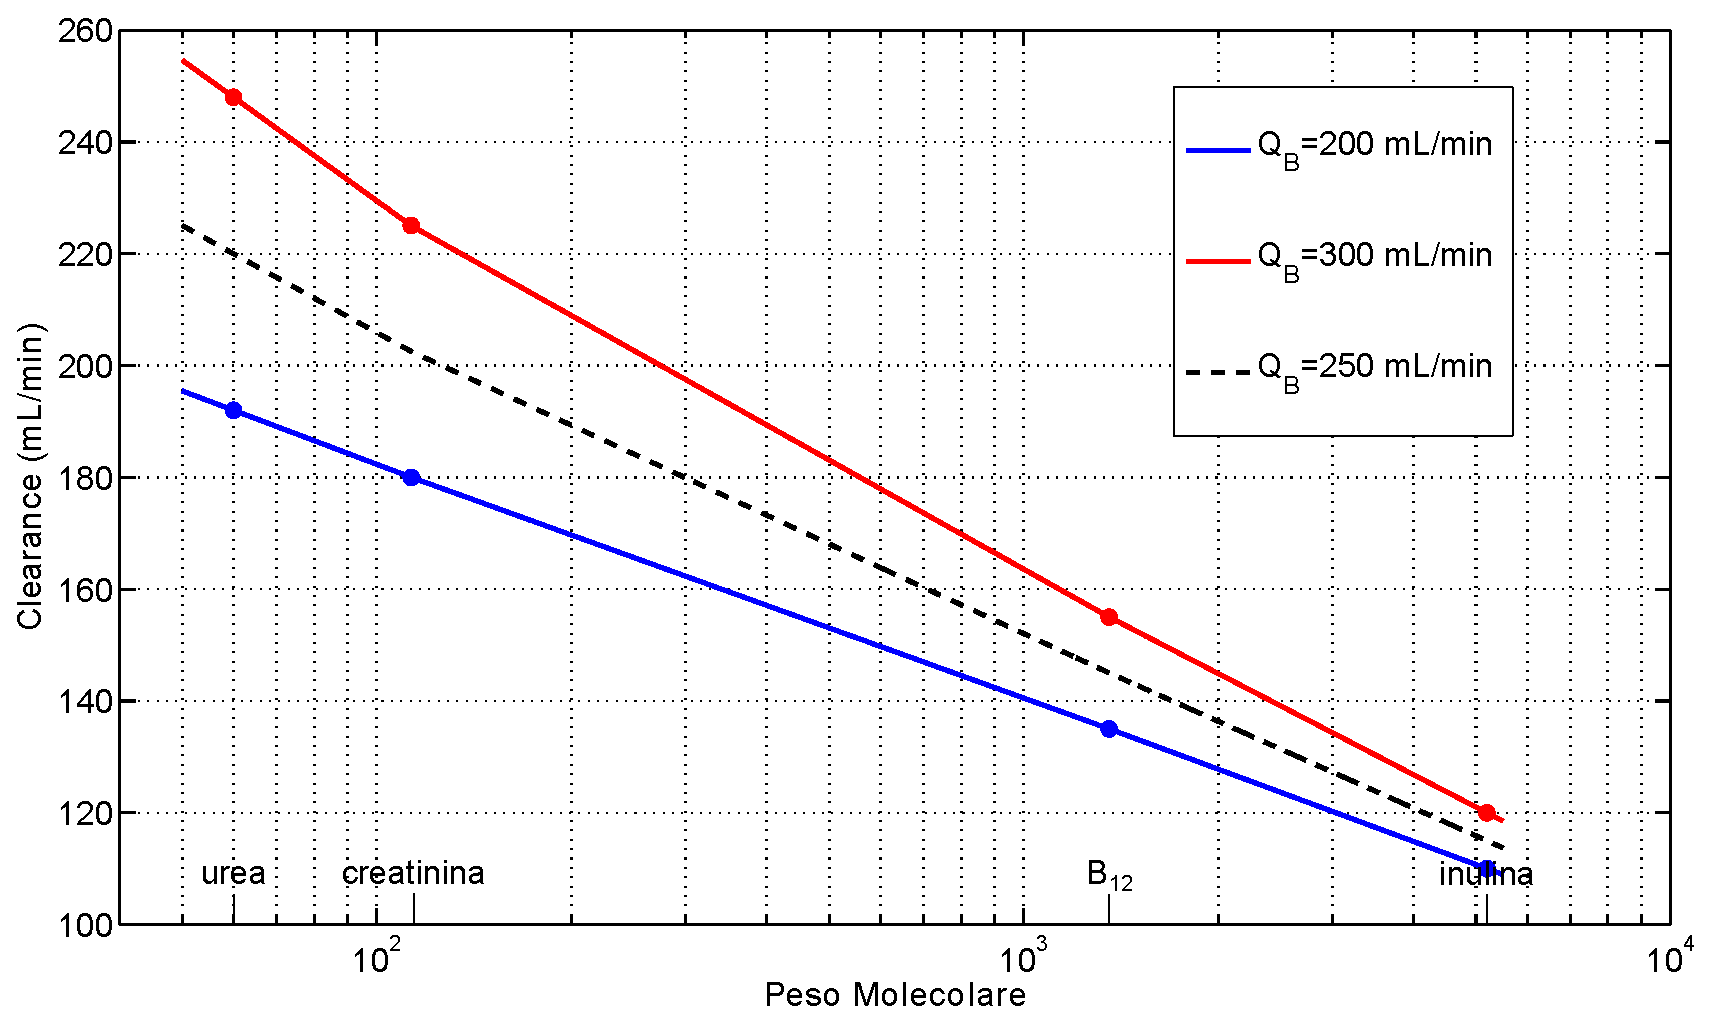
\includegraphics[width=0.9\textwidth]{immagini/interp_log.eps}
		\caption{Clearance del filtro HF80s, in regime di filtrazione nulla ($Q_f=0$).}
		\label{fig:doppia_interp}
\end{figure}
La portata volumetrica in ingresso al dializzatore è calcolata nel seguente modo:
\begin{align*}
	Q_B &= Q_{fistola} \quad\text{, in POST-diluizione}\\
	Q_B &= Q_{fistola} + Q_s \quad\text{, in PRE-diluizione}
\end{align*}
dove $Q_s$ è la portata del fluido di diluizione.

\section{Coefficienti di Staverman - $\sigma$}
Nell'Eq.~(\ref{phit}) che descrive il flusso convettivo attraverso la membrana del dializzatore, compare il fattore di \textit{hindrance} $\varepsilon$. Il complemento a uno di $\varepsilon$ è chiamato \textit{coefficiente di riflessione}, o di \textit{Staverman}, e si indica con la lettera $\sigma$. Da correlazioni sperimentali \cite{Liao} si ricava che:
\begin{equation}
	\sigma _s = \bigl(1-(1-r_s/r_p)^2\bigr)^2
	\label{eq:staverman}
\end{equation}
dove $r_s/r_p$ è il rapporto fra il raggio del soluto $s$ e del poro della membrana.
In Liao et al. \cite{Liao} si trova che per l'inulina ($r_s=1,47$ $nm$) il filtro HF80s ha un coefficiente $\sigma _s$ pari a $0,56$. Da questi dati, usando l'Eq.~(\ref{eq:staverman}), possiamo ricavare il raggio (medio efficace) dei pori del filtro HF80s. Successivamente, conoscendo il raggio dei soluti che vogliamo introdurre nel modello, possiamo usare la stessa formula per calcolare il loro coefficiente di riflessione. Il risultato del calcolo è mostrato in \tablename~\ref{tab:staverman}, in cui i valori dei raggi delle molecole sono stati in parte ricavati dal testo di fisiologia di Boron \cite{boron}.

\begin{table}[htb]
	\centering
	\caption{Calcolo di $\sigma$ per alcuni soluti}\label{tab:staverman}
		\begin{tabular}{lccc}
\toprule
Soluto      & $r_s$  & $\sigma_s$ & $(1-\sigma_s)$ \\
            & $(pm)$ &            &                \\
\midrule
$Na^+$      & $100$  & $0,004$      & $0,996$      \\
$K^+$       & $140$  & $0,009$      & $0,991$      \\
$Cl^-$      & $180$  & $0,014$      & $0,986$      \\
$HCO_3^-$   & $156$  & $0,010$      & $0,990$      \\
$Ca^{++}$   & $100$  & $0,004$      & $0,996$      \\
$Mg^{++}$   &{ }$72$ & $0,002$      & $0,998$      \\
$PO_4^{3-}$ & $238$  & $0,024$      & $0,976$      \\
Urea        & $160$  & $0,011$      & $0,989$      \\
Creatina    & $300$  & $0,036$      & $0,964$      \\
Glucosio    & $330$  & $0,045$      & $0,955$      \\
Albumina    &$3550$  & $0,919$      & $0,081$      \\
\bottomrule
\end{tabular}
\end{table}

\section{Coefficienti di Donnan - $\alpha_d$}
L'effetto Donnan è dovuto principalmente all'impermeabilità attraverso una membrana porosa di alcuni soluti elettricamente carichi. Poiché sono le proteine ad essere la causa preponderante di questo effetto e poiché sia la membrana capillare che quella del dializzatore sono entrambi impermeabili alle proteine, possiamo ipotizzare che il coefficiente $\alpha_d$ che compare nell'equazione che descrive il flusso di massa attraverso il dializzatore, e il coefficiente $\alpha_d$ che compare nell'equazione che descrive il flusso di massa verso il compartimento intracellulare, abbiano gli stessi valori numerici calcolati con l'Eq.~(\ref{eq:donnan}) riproposta qui di seguito:
\begin{equation}
	\alpha_d = \frac{\alpha-1}{7} \cdot T_p + 1 \qquad \text{con} \qquad \alpha=\frac{C_{is,eq}}{C_{pl,eq}}
\end{equation}
in cui i valori di equilibrio sono presi dalla \tablename~\ref{tab:osmolarit}. Bisogna fare attenzione alla concentrazione di proteine totali $T_p$ da inserire nell'equazione. Mentre nel caso della post-diluizione si utilizza la stessa concentrazione plasmatica, nel caso della PRE-diluizione bisogna tener conto del fatto che il liquido in ingresso al dializzatore sarà diluito in proporzione pari alla portata di diluizione, e pertanto si avrà una concentrazione di proteine totali minore rispetto a quella plasmatica, da calcolare con un opportuno bilancio di massa.


